\documentclass[12pt,a4paper]{article}
% The \documentclass command specifies the nature of the document: article, report, book, memoir are the most common
% Within square brackets [ ] you call options: in this case 12pt is for setting the font size to 12 points, a4paper is for setting the paper size to A4
% Paragraphs starting with the percentage symbol % are comments and do not appear in the final document

\usepackage{graphicx}
\usepackage{tikz} % for drawing
    \usetikzlibrary{trees}
\usepackage[hidelinks]{hyperref} % hyperlinks in the PDF

\usepackage{fontspec}
    \setmainfont{Times New Roman} % horrible typeface, don't use it if you can
\usepackage{polyglossia}
    \setmainlanguage{english}

% The command \usepackage adds extra-functionalities through packages. This command can be used *only* in the preamble
% graphicx is for figures, fontspec is for choosing the typeface, polyglossia for setting the language of your document

\usepackage{ctable} % this is for tables, check the documentation

\usepackage[numbers]{natbib}
%\usepackage{natbib} % for Harvard referencing

\title{My first document}
\author{Me}
\date{4 February 2016}

% if you use \date{} instead, no date is typeset

\begin{document}

\maketitle
\tableofcontents

% The content of the document itself must be within \begin{document} and \end{document}. The commands \begin and \end create an "environment". The document environment is essential!
% \maketitle calls the title
% \tableofcontents creates the table of contents

\section{Introduction}
\label{s:introduction}
Call me Ishmael. Some years ago---never mind how long precisely---having little or no money in my purse, and nothing particular to interest me on shore, I thought I would sail about a little and see the watery part of the world. It is a way I have of driving off the spleen and regulating the circulation. Whenever I find myself growing grim about the mouth; whenever it is a damp, drizzly November in my soul; whenever I find myself involuntarily pausing before coffin warehouses, and bringing up the rear of every funeral I meet; and especially whenever my hypos get such an upper hand of me, that it requires a strong moral principle to prevent me from deliberately stepping into the street, and methodically knocking people's hats off---then, I account it high time to get to sea as soon as I can.\footnote{This is how you create a footnote.}

\subsection{Methods}

This is my substitute for \textit{pistol} and \textbf{ball}. With a philosophical flourish \textbf{\textit{Cato}} throws himself upon his sword; I quietly take to the ship. There is nothing surprising in this. If they but knew it, almost all men in their degree, some time or other, cherish very nearly the same feelings towards the ocean with me.

\begin{itemize}
    \item This is just a list
    \item with some random text
    \item if you don't mind
\end{itemize}

This is my substitute for pistol and ball. With a philosophical flourish Cato throws himself upon his sword; I quietly take to the ship. There is nothing surprising in this. If they but knew it, almost all men in their degree, some time or other, cherish very nearly the same feelings towards the ocean with me.

\begin{enumerate}
    \item This is another list
    \item but with numbers
\end{enumerate}

This is my substitute for pistol and ball. With a philosophical flourish Cato throws himself upon his sword; I quietly take to the ship. There is nothing surprising in this. If they but knew it, almost all men in their degree, some time or other, cherish very nearly the same feelings towards the ocean with me.

\begin{enumerate}
    \item This is yet another
    \item but with multiple levels
    \begin{enumerate}
        \item List in a list
        \item second item
    \end{enumerate}
    \item End of the list
\end{enumerate}

% Figures are included with the "figure" environment

\begin{figure}
    \centering
    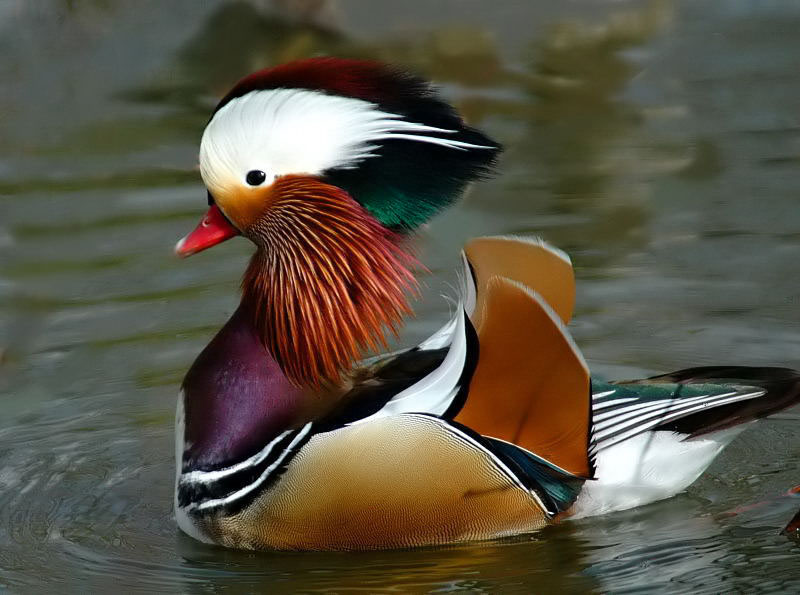
\includegraphics[width=0.6\textwidth]{mandarin_duck.jpg}
    \caption{A mandarin duck.}
    \label{f:duck}
\end{figure}

Call me Ishmael. Some years ago---never mind how long precisely---having little or no money in my purse, and nothing particular to interest me on shore, I thought I would sail about a little and see the watery part of the world. It is a way I have of driving off the spleen and regulating the circulation. Whenever I find myself growing grim about the mouth; whenever it is a damp, drizzly November in my soul; whenever I find myself involuntarily pausing before coffin warehouses, and bringing up the rear of every funeral I meet; and especially whenever my hypos get such an upper hand of me, that it requires a strong moral principle to prevent me from deliberately stepping into the street, and methodically knocking people's hats off---then, I account it high time to get to sea as soon as I can.

\ctable[caption = My table.,
label= t:simple
]{ll}{}{
\FL
\textbf{yes} & \textbf{no} \ML
10 & 9 \LL
}

\subsubsection{A subsubsection}

Call me Ishmael. Some years ago---never mind how long precisely---having little or no money in my purse, and nothing particular to interest me on shore, I thought I would sail about a little and see the watery part of the world. It is a way I have of driving off the spleen and regulating the circulation. Whenever I find myself growing grim about the mouth; whenever it is a damp, drizzly November in my soul; whenever I find myself involuntarily pausing before coffin warehouses, and bringing up the rear of every funeral I meet; and especially whenever my hypos get such an upper hand of me, that it requires a strong moral principle to prevent me from deliberately stepping into the street, and methodically knocking people's hats off---then, I account it high time to get to sea as soon as I can.

\ctable[caption = My second table.,
label= t:complex
]{lll}{}{
\FL
& yes & no \ML
first pool & 10 & 9 \NN
second pool & 15 & 3 \LL
}

Call me Ishmael. Some years ago---never mind how long precisely---having little or no money in my purse, and nothing particular to interest me on shore, I thought I would sail about a little and see the watery part of the world. It is a way I have of driving off the spleen and regulating the circulation. Whenever I find myself growing grim about the mouth; whenever it is a damp, drizzly November in my soul; whenever I find myself involuntarily pausing before coffin warehouses, and bringing up the rear of every funeral I meet; and especially whenever my hypos get such an upper hand of me, that it requires a strong moral principle to prevent me from deliberately stepping into the street, and methodically knocking people's hats off---then, I account it high time to get to sea as soon as I can.

\section{Maths}

I love Maths! $\int_0^\infty \mathrm{e}^{-x}\,\mathrm{d}
x$.
\begin{equation}
    \cos (2\theta) = \cos^2 \theta - \sin^2 \theta
\end{equation}

Call me Ishmael. Some years ago---never mind how long precisely---having little or no money in my purse, and nothing particular to interest me on shore, I thought I would sail about a little and see the watery part of the world.

\begin{equation}
    \sqrt[n]{1+x+x^2+x^3+\ldots}
\end{equation}

Call me Ishmael. Some years ago---never mind how long precisely---having little or no money in my purse, and nothing particular to interest me on shore, I thought I would sail about a little and see the watery part of the world.

\begin{equation}\label{e:yoyo}
    \sum_{i=1}^{10} t_i
\end{equation}

\section{Cross-referencing}
As I said in Section \ref{s:introduction}, you can call me Ishmael. An example of vote counting is shown in Table \ref{t:complex}. Figure \ref{f:duck} is a picture of a mandarin duck. In equation \ref{e:yoyo}.

\section{How to reference}

\begin{figure}
\tikzstyle{every node}=[draw=black,thick,anchor=west]
\centering
\begin{tikzpicture}[%
  grow via three points={one child at (0.5,-0.7) and
  two children at (0.5,-0.7) and (0.5,-1.4)},
  edge from parent path={(\tikzparentnode.south) |- (\tikzchildnode.west)}]
  \node {texmf}
    child { node {tex} }				
    child { node {bibtex}
        child { node {bib} }
        child { node {bst} }
    };
\end{tikzpicture}
  \caption{The \texttt{texmf} folder structure.}
  \label{f:texmf}
\end{figure}

Put your \texttt{.bib} files inside the \texttt{bib} folder of your \texttt{texmf folder} (see folder structure in Figure \ref{f:texmf}). Put your \texttt{.bst} files inside the \texttt{bst} folder. I am providing here a sample \texttt{.bib}: you don't need to move this to the \texttt{bib} folder, it is just a sample.

Some examples: \citet{capra1983}, \citep{dunleavy2003}, \citep[p. 1--10]{medina2008}. An interesting quotation from \citet[p. 4--5]{medina2008}:

\begin{quotation}
What we know about the brain comes from biologists who study brain tissues, experimental psychologists who study behavior, cognitive neuroscientists who study how the first relates to the second, and evolutionary biologists. Though we know precious little about how the brain works, our evolutionary history tells us this: The brain appears to be designed to solve problems related to surviving in an unstable outdoor environment, and to do so in nearly constant motion. I call this the brain’s performance envelope.
\end{quotation}


% If you want to know more, go to https://en.wikibooks.org/wiki/LaTeX and read the wikibook!

% Happy TeXing!

\bibliographystyle{plainnat}
%\bibliographystyle{dcu} % for Harvard referencing style
\bibliography{library}

\end{document}
